\documentclass[12pt]{article}
\usepackage[utf8]{inputenc}
\usepackage{amsmath, amssymb, amsthm, graphicx, fancyvrb, enumitem, titlesec, setspace, float, fancyvrb}
\usepackage[dvipsnames]{xcolor}
\usepackage[top=1in, bottom=1in, left=1.25in, right=1.25in]{geometry}
\titleformat{\section}{\normalfont\bfseries}{}{0em}{}
\titlespacing*{\section}{0pt}{1.5ex plus .2ex minus .2ex}{0.8ex plus .1ex}


\begin{document}
\noindent Andre Winkel \hfill \today \\
\rule{\textwidth}{0.4pt} \vspace{0em}
\begin{center} \large{Lab 2} \end{center} \vspace*{0em}

\section*{Problem 1: Simulating reverberations}
In this problem, we will simulate reverberations using an audio clip.
\begin{enumerate}[label=\textbf{\alph*)}, leftmargin=2.6em]

\item Loading the clip and plotting the signal, we observe the plot below:
\begin{figure}[H]
    \centering
    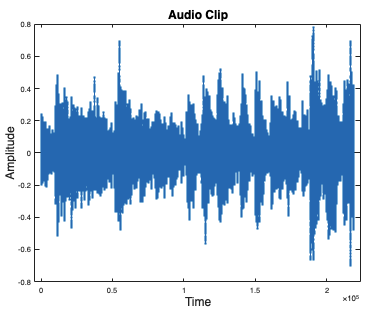
\includegraphics[width=0.5\linewidth]{plot1.png}
\end{figure}
\begin{Verbatim}[frame=single, commandchars=\\\{\}]
>> [audio_clip , fs] = audioread(\textcolor{violet}{'ee110b.m4a'});
>> audio_clip = mean(audio_clip, 2);  \textcolor{Green}{% stereo to mono}
>> \textcolor{blue}{sound}(audio_clip, fs);
>> stem(audio_clip, (\textcolor{violet}{'.'});
>> title(\textcolor{violet}{"Audio Clip"}, \textcolor{violet}{"FontSize"}, 16);
>> xlabel(\textcolor{violet}{"Time"}, \textcolor{violet}{"FontSize"}, 16);
>> ylabel(\textcolor{violet}{"Amplitude}, \textcolor{violet}{"FontSize"}, 16);
\end{Verbatim}

\item Given that audio reverberations can be written as a sum of delayed and scaled copies of the original signal,
\begin{equation}
    y[n] = \sum_{k=0}^{N_\text{reverb}-1} a_{qk}x[n-q_k],
\end{equation}
by definition, we can conclude the impulse response must be
\begin{equation}
    h[n] = \sum_{k=0}^{N_\text{reverb}-1} a_{qk}\delta[n-q_k]
\end{equation}
as this is a discrete-time LTI system. This is a series of time-shifted and scaled impulses. As $h[n]$ is a finite sum of scaled impulses, finite values, the condition for stability,
\begin{equation}
    \sum_{n=-\infty}^\infty |h[n]| < \infty, \rightarrow \sum_{k=0}^{N_\text{reverb}-1} a_{qk}< \infty,
\end{equation}
is true. Therefore, we can conclude that the system is stable.

\item The plot of an impulse response with $N_\text{reverb}=10$, $y[n]$ of length $10,000$, $q_k=1000k$, and $a_{qk}=[\frac{1}{2}]^k$ is shown below:
\begin{figure}[H]
    \centering
    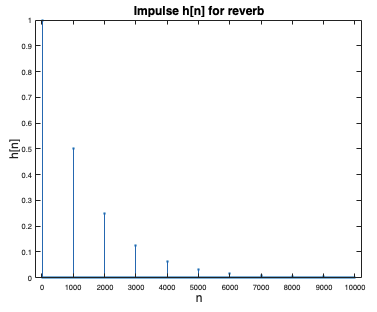
\includegraphics[width=0.5\linewidth]{plot2.png}
\end{figure}
\begin{Verbatim}[frame=single, commandchars=\\\{\}]
>> h_reverb = zeros(10000, 1);

>> \textcolor{blue}{for} k = 0:9
>> qk = 1000 * k;      \textcolor{Green}{% delay pos}
>> ak = 1 / (2^k);
>> h_reverb(qk+1) = ak;  \textcolor{Green}{% index adjust}
>> \textcolor{blue}{end}

>> stem(h_reverb, \textcolor{violet}{'.'});
>> title(\textcolor{violet}{'Impulse h[n] for reverb'}, \textcolor{violet}{'FontSize'}, 16);
>> xlabel(\textcolor{violet}{'n'}, \textcolor{violet}{'FontSize'}, 16);
>> ylabel(\textcolor{violet}{'h[n]'}, \textcolor{violet}{'FontSize'}, 16);
\end{Verbatim}

\item The output for this system, $y[n]=x[n]\ast h[n]$, is shown below:
\begin{figure}[H]
    \centering
    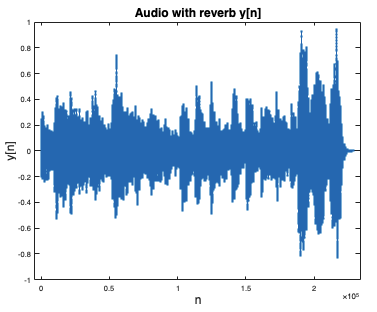
\includegraphics[width=0.5\linewidth]{plot3.png}
\end{figure}
\begin{Verbatim}[frame=single, commandchars=\\\{\}]
>> reverb_audio = conv(audio_clip, h_reverb);
>> \textcolor{blue}{sound}(reverb_audio, fs);
>> \textcolor{blue}{stem}(reverb_audio, \textcolor{violet}{'.'});
>> \textcolor{blue}{title}(\textcolor{violet}{'Audio with reverb y[n]'}, \textcolor{violet}{'FontSize'}, 16);
>> \textcolor{blue}{xlabel}(\textcolor{violet}{'n'}, \textcolor{violet}{'FontSize'}, 16);
>> \textcolor{blue}{ylabel}(\textcolor{violet}{'y[n]'}, \textcolor{violet}{'FontSize'}, 16);
\end{Verbatim}

\item The output for the system with $a_{qk}=0.7^k$ is shown below:
\begin{figure}[H]
    \centering
    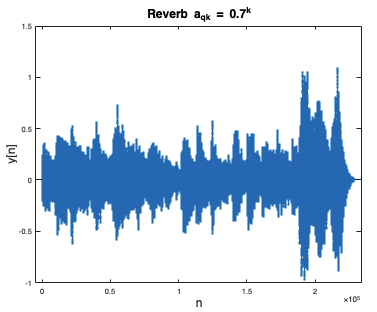
\includegraphics[width=0.5\linewidth]{plot4.png}
\end{figure}
\begin{Verbatim}[frame=single, commandchars=\\\{\}]
>> h_reverb = zeros(10000, 1);

>> \textcolor{blue}{for} k = 0:9
>> qk = 1000 * k;
>> ak = 0.7^k;
>> h_reverb(qk+1) = ak;
>> \textcolor{blue}{end}

>> reverb_audio = conv(audio_clip, h_reverb);
>> \textcolor{blue}{sound}(reverb_audio, fs);
>> \textcolor{blue}{stem}(reverb_audio, \textcolor{violet}{'.'});
>> \textcolor{blue}{title}(\textcolor{violet}{'Reverb a_{qk} = 0.7^k'}, \textcolor{violet}{'FontSize'}, 16);
>> \textcolor{blue}{xlabel}(\textcolor{violet}{'n'}, \textcolor{violet}{'FontSize'}, 16);
>> \textcolor{blue}{ylabel}(\textcolor{violet}{'y[n]'}, \textcolor{violet}{'FontSize'}, 16);
\end{Verbatim}
When compared to the original audio with reverb in part \textbf{d)}, we find that the signal has higher peaks in amplitude. It almost looks like the reverberations closely follow the original signal, even though they should, in practice, be further in distance. When listening to this sample, it sounds much more distorted as well, and is much more unpleasant to listen to \---- it more closely resembles a "chorus" effect as opposed to a reverb one, though it is important to consider that they are very similar, only different in the parameter that was changed for this example.

\item Repeating the experiment with $q_k=2000k, N_\text{reverb}=5$ and $a_{qk}=[\frac{1}{2}]^k$, we achieve the plot below:
\begin{figure}[H]
    \centering
    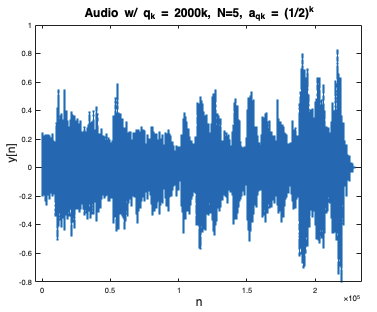
\includegraphics[width=0.5\linewidth]{plot5.png}
\end{figure}
\begin{Verbatim}[frame=single, commandchars=\\\{\}]
>> h_reverb = zeros(10000, 1);

>> \textcolor{blue}{for} k = 0:4
>> qk = 2000 * k;
>> ak = 1 / (2^k);
>> h_reverb(qk+1) = ak;
>> \textcolor{blue}{end}

>> reverb_audio = conv(audio_clip, h_reverb);
>> \textcolor{blue}{sound}(reverb_audio, fs);
>> \textcolor{blue}{stem}(reverb_audio, \textcolor{violet}{'.'});
>> \textcolor{blue}{title}(\textcolor{violet}{'Audio w/ q_k = 2000k, N=5, a_{qk} = (1/2)^k'}, 
\textcolor{violet}{'FontSize'}, 16);
>> \textcolor{blue}{xlabel}(\textcolor{violet}{'n'}, \textcolor{violet}{'FontSize'}, 16);
>> \textcolor{blue}{ylabel}(\textcolor{violet}{'y[n]'}, \textcolor{violet}{'FontSize'}, 16);
\end{Verbatim}
This audio clip looks and sounds very similar to the original we had produced. The reason for this is that while $q_k$ has increased by a factor of $2$, $N_\text{reverb}$ has decreased by a factor of $2$. In practice, this means that they essentially cancel each other out, and we are left with the same signal that we started with. That is, the signal sounds more like a realistic replication of what reverberations in a larger room would sound compared to the previous example.
\end{enumerate}


\section*{Problem 2: Difference equations}
In this problem, we consider a system described by the following difference equation:
\begin{equation}
    y[n] = \frac{1}{2} y[n-1] + x[n].
\end{equation}
We let $x[n]=1$, and assume the initial condition $y[0]=0$.

\begin{enumerate}[label=\textbf{\alph*)}, leftmargin=2.6em]
\item Evaluating $y[n]$ for $n=0,1,2,...,100$, we obtain the following plot of output $y[n]$ for all values of $n$:
\begin{figure}[H]
    \centering
    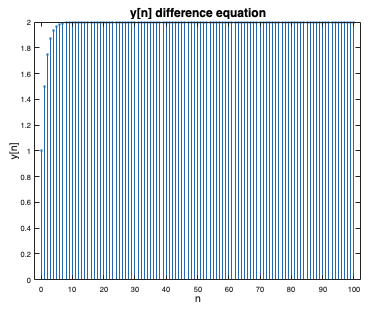
\includegraphics[width=0.5\linewidth]{plot6.png}
\end{figure}
\begin{Verbatim}[frame=single, commandchars=\\\{\}]
>> n = 0:100; \textcolor{Green}{% Time axis}
>> x = ones(1, 101); \textcolor{Green}{% Input signal}
>> y = zeros(1, 101); \textcolor{Green}{% Output}
>> 
>> \textcolor{blue}{for} idx = 1:length(n)
>>     \textcolor{blue}{if} idx == 1
>>         y(idx) = x(idx);
>>     \textcolor{blue}{else}
>>         y(idx) = 0.5 * y(idx - 1) + x(idx);
>>     \textcolor{blue}{end}
>> \textcolor{blue}{end}
>> 
>> \textcolor{blue}{stem}(n, y, \textcolor{violet}{'.'});
>> \textcolor{blue}{title}(\textcolor{violet}{'Output y[n] from difference equation'}, \textcolor{violet}{'FontSize'}, 16);
>> \textcolor{blue}{xlabel}(\textcolor{violet}{'n'}, \textcolor{violet}{'FontSize'}, 14);
>> \textcolor{blue}{ylabel}(\textcolor{violet}{'y[n]'}, \textcolor{violet}{'FontSize'}, 14);
\end{Verbatim}

\item Considering an LTI system with the impulse response, $h[n]=\frac{1}{2^n}u[n]$, we will evaluate and plot the step response of the system below:
\begin{figure}[H]
    \centering
    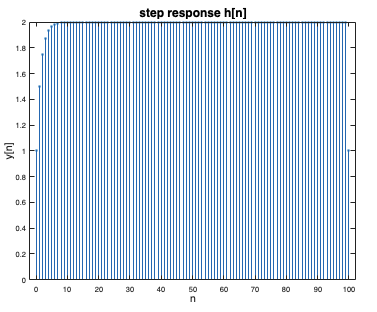
\includegraphics[width=0.5\linewidth]{plot7.png}
\end{figure}
\begin{Verbatim}[frame=single, commandchars=\\\{\}]
>> n = 0:100; \textcolor{Green}{% time axis}
>> h = (1/2).^n; \textcolor{Green}{% impulse response}
>> x = ones(1, 100); \textcolor{Green}{% step input}
 
>> y_step = conv(x, h);
>> y_step = y_step(1:101); \textcolor{Green}{% length match}
 
>> \textcolor{blue}{stem}(n, y_step, \textcolor{violet}{'.'});
>> \textcolor{blue}{title}(\textcolor{violet}{'step response h[n]'}, \textcolor{violet}{'FontSize'}, 16);
>> \textcolor{blue}{xlabel}(\textcolor{violet}{'n'}, \textcolor{violet}{'FontSize'}, 14);
>> \textcolor{blue}{ylabel}(\textcolor{violet}{'y[n]'}, \textcolor{violet}{'FontSize'}, 14);
\end{Verbatim}

\item The systems described in \textbf{a)} and \textbf{b)} are the same. This is primarily indicated by their resulting output being the same. We can prove this by setting the input $x[n] = \delta[n]$ and analyzing the output $y[n]$. Applying this, we see
\[
\begin{aligned}
y[0] &= \delta[0] = 1 \\
y[1] &= \frac{1}{2}y[0] + \delta[1] = \frac{1}{2} \\
y[2] &= \frac{1}{2}y[1] + \delta[2] = \frac{1}{4} \\
y[3] &= \frac{1}{2}y[2] + \delta[3] = \frac{1}{8} \\
&\vdots \\
y[n] &= \frac{1}{2^n}u[n].
\end{aligned}
\]
This indicates that the systems are equal, as we can obtain the impulse response from the difference equation.
\end{enumerate}
\end{document}